% !TEX root = main.tex

\section{不确定性规划}
% Bayesian networks: graphs + tables, inference
% Variable elimination algorithm
% Use D-separation to determine independence

\subsection{基础知识}
一组变量$V_1,\ldots,V_n$以及其对应的有限域$\dom[V_i]$,很容易导致指数的计算复杂度。
\begin{theorem}[全概率公式]
$\{B\}_{i=1}^k$为全集$U$的一个划分,则
\[\begin{aligned}
\pr{A}&=\pr{A\cap B_1}+\cdots+\pr{A\cap B_k}\\
&=\pr{A\mid B_1}\pr{B_1}+\cdots+\pr{A\mid B_k}\pr{B_k}
\end{aligned}\]
\end{theorem}
\begin{theorem}[条件独立]
若
\[\pr{B\mid A\cap C}=\pr{B\mid A}\]
,则在给定$A$的情况下$B$条件独立于$C$($C$没有给$A$增加知识)。
若对于所有$x\in\dom[X],y\in\dom[Y],z\in\dom[Z]$,
\[\pr{X=x\land Y=y\mid Z=z}=\pr{X=x\mid Z=z}\pr{Y=y\mid Z=z}\]
则在给定$Z=z$下,$X=x$和$Y=y$条件独立。
\end{theorem}
\begin{proposition}[独立性性质]
\begin{itemize}
	\item 若$A$和$B$独立,则$\pr{A\cap B}=\pr{A}\cdot\pr{B}$
	\item 给定$A$,$B$和$C$条件独立,则
	\[\pr{B\cap C\mid A}=\pr{B\mid A}\pr{C\mid A}\]
\end{itemize}
\end{proposition}
\begin{theorem}[贝叶斯公式]
条件概率定义
\[\pr{X\mid Y}=\pr{XY}/\pr{Y}\implies \pr{XY}=\pr{X\mid Y}\pr{Y}\]
注意与贝叶斯公式区分
\[\pr{Y\mid X}=\frac{\pr{XY}}{\pr{X}}=\frac{\pr{X\mid Y}\pr{Y}}{\pr{X}}\]
\end{theorem}
\begin{theorem}[链式法则]
\[\pr{A_1\cap A_2\cap\cdots\cap A_n}=\pr{A_1\mid A_2\cap\cdots\cap A_n}\pr{A_2\mid A_3\cdots\cap A_n}\pr{A_{n-1}\mid A_n}\pr{A_n}\]
% P(123) = P(1|23)P(2|3)P(3) = P(123)/P(23) P(23)/P(3) P(3)
\end{theorem}

\subsection{贝叶斯网络}
\subsubsection{基础知识}
\begin{bayesian}
E \arrow[r] & C\arrow[r] & A \arrow[r] & B\arrow[r] & H
\end{bayesian}
有以下概率公式成立
\begin{itemize}
	\item $\pr{H\mid B,A,E,C}=\pr{H\mid B}$
	\item 由链式法则和独立性假设
	\[\begin{aligned}
		\pr{HBACE}&=\pr{H\mid BACE}\pr{B\mid ACE}\pr{A\mid CE}\pr{C\mid E}\pr{E}\\
		\pr{HBACE}&=\pr{H\mid B}\pr{B\mid A}\pr{A\mid C}\pr{C\mid E}\pr{E}
	\end{aligned}\]
	\item 通用公式
	\[\pr{X_1X_2\cdots X_n}=\pr{X_n\mid Par(X_n)}\cdots\pr{X_1\mid Par(X_1)}\]
	\item 单点概率(由全概率公式和条件概率定义)
	\[\begin{aligned}
		\pr{a}&=\sum_{c_i\in\dom[C]}\pr{a\mid c_i}\pr{c_i}\\
		&=\sum_{c_i\in\dom[C]}\pr{a\mid c_i}\sum_{e_i\in\dom[E]}\pr{c_i\mid e_i}\pr{e_i}
	\end{aligned}\]
\end{itemize}

因此每个结点只需存一个条件概率表(conditional probability table, CPT)。

\begin{definition}[D分隔(separation)]
若一组变量$E$阻隔(block)了$X$到$Y$的所有\textcolor{red}{无向路径}$P$,则称$E$ D-分隔了$X$和$Y$,且有给定证据$E$下,$X$和$Y$条件独立。
$E$阻隔了路径$P$当且仅当在路径上存在某点$Z$使得下面任一成立:(一定要小心箭头方向)
\begin{figure}[H]
\centering
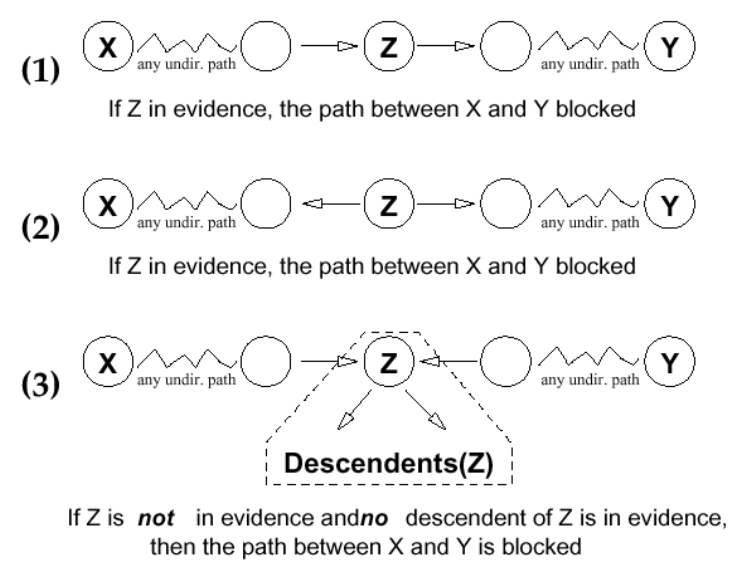
\includegraphics[width=0.8\linewidth]{fig/blocking.png}
\end{figure}
注意第3种情况,\textemph{交叉结点及其子结点都没有在证据集中给出},则父亲节点被阻隔。
\end{definition}
\begin{example}
考虑如下贝叶斯网络
\begin{bayesian}
A\arrow[dr] & & B\arrow[dl] \arrow[dr] & \\
 & C\arrow[dl] \arrow[dr] & & D\\
E & & F &
\end{bayesian}
在此例中$\pr{c\mid a,b,\lnot d,\lnot e,\lnot f}\ne\pr{c\mid a,b}$,要求前者还是拿条件概率展开为全变元非条件概率来求解。
\end{example}
\begin{example}
考虑下图的贝叶斯网络
\begin{figure}[H]
\centering
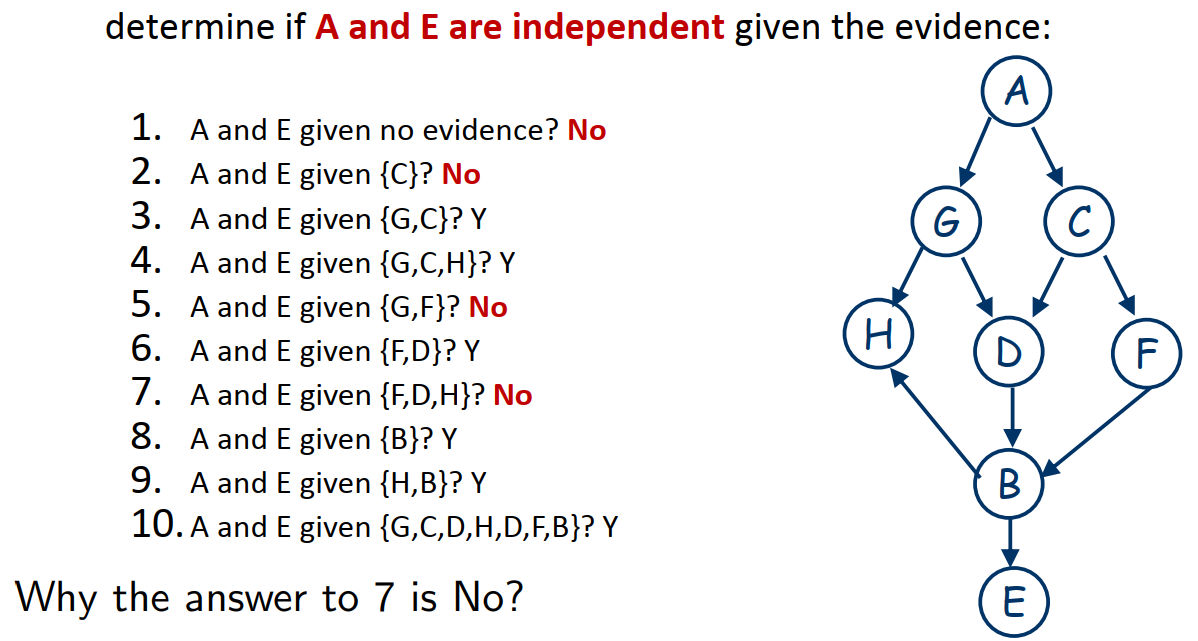
\includegraphics[width=0.8\linewidth]{fig/d-separation_example.png}
\end{figure}
注意第3种情况的适用条件,由于$H$在证据集中,所以并不满足第3种情况。
在第7个例子中,$AGHBE$没有被阻隔,故给定$FDH$,$A,E$也不独立。
\end{example}

\subsubsection{贝叶斯推断}
推断过程如下:
\[\begin{aligned}
\pr{a\mid d,e}&=\pr{a,d,e}/\pr{d,e}\\
&=\pr{a,d,e}/\sum_{A}\pr{a,d,e}\\
\pr{a,d,e}&=\sum_{B,C}\pr{a,B,C,d,e}
\end{aligned}\]
故只需计算$\pr{a,d,e}$。

采用动态规划的思想,存储子项,减少计算量。

记因子为某些变量的函数,如$\pr{C\mid A}=f(A,C)$
\begin{itemize}
	\item 乘积:$h(X,Y,Z)=f(X,Y)\times g(Y,Z)$
	\item 求和:$h(Y)=\sum_{x\in\dom[X]}f(x,Y)$
	\item 因子限定:$h(Y)=f(a,Y)$
\end{itemize}

\begin{myalgorithm}[变量消除(Variable Elimination, VE)]
给定贝叶斯网络,条件概率表$F$,询问$Q$,证据$E$,其余变量为$Z$,计算$\pr{Q\mid E}$。
\begin{enumerate}
	\item 对于$f\in F$中每一变量,将其替换为$f_{E=e}$(因子限定)
	\item 对于每一$Z_j\in Z$,按给定$Z_j$顺序,并按照以下步骤消除:
	\begin{itemize}
		\item $f_1,f_2,\ldots,f_k$为含有$Z_j$的因子
		\item 计算新的因子$g_j=\sum_{Z_j}f_1\times f_2\times\cdots\times f_k$
		\item 将$f_i$从$F$中移除,并将新的因子$g_j$添加到$F$中
	\end{itemize}
	\item 剩下的因子只包含询问$Q$中的变量,则计算它们的乘积归一化得到$\pr{Q\mid E}$
\end{enumerate}
\end{myalgorithm}

可以采用桶消除(bucket elimination)算法,每次将新生成的因子放在第一个可被应用的桶中。
下图展示的是超图(hypergraph),最大超边(hyperedge)的大小即为最大的CPT表项/VE算法的复杂度。
\begin{figure}[H]
\centering
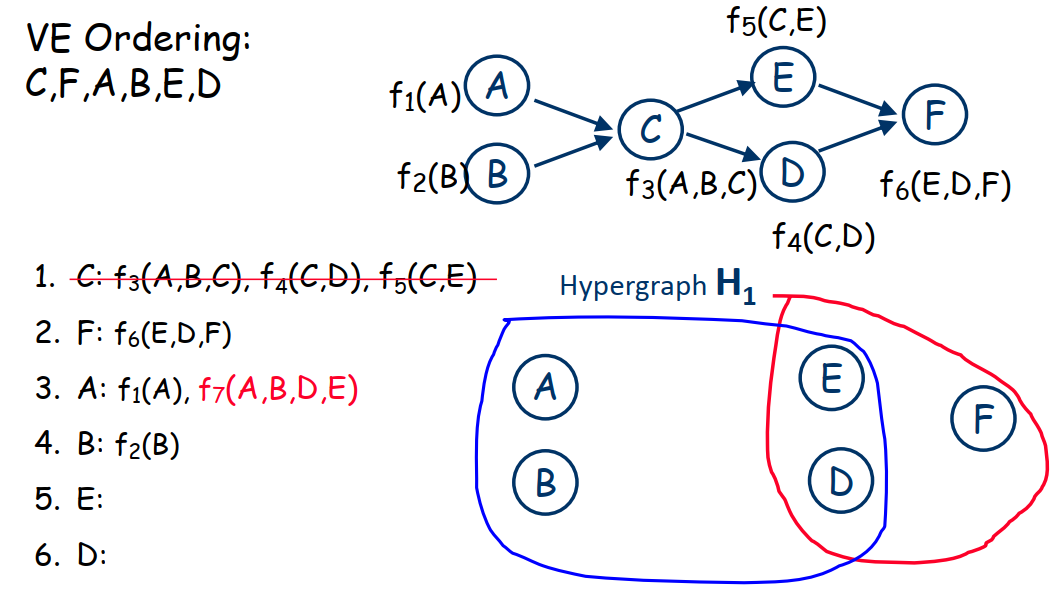
\includegraphics[width=0.8\linewidth]{fig/bucket_elimination.png}
\end{figure}

多树(polytree):单连通(singly connected)的贝叶斯网络,即在任意两个结点间只有一条路径。

最小填充(min-fill)启发式:总是先消除产生最小因子大小的变量,这种方法可以使得在线性时间内求解多树。

\begin{definition}[相关性(relevance)]
给定证据$E$询问$Q$,则有以下几种情况:
\begin{itemize}
	\item $Q$自身当然是相关的
	\item 若结点$Z$相关,则它的父母也相关
	\item 若\textcolor{red}{$e\in E$}是一个相关结点的\textcolor{red}{后代},则$E$也是相关的
\end{itemize}
\end{definition}
\begin{example}
若询问$P(F\mid H)$,则$D,E,G$是不相关的,这种算法会过度估计相关的变量。
\begin{figure}[H]
\centering
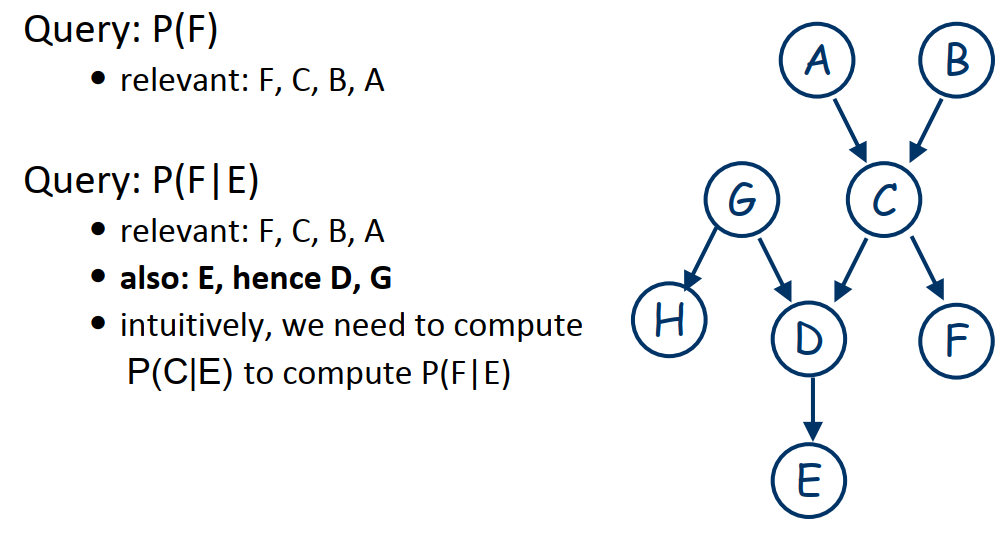
\includegraphics[width=0.8\linewidth]{fig/relevance_example.png}
\end{figure}
\end{example}